\documentclass[11pt,a4paper]{article}

\usepackage{amsfonts}
\usepackage[centertags]{amsmath}
\usepackage{amsthm}
\usepackage{amssymb}

\usepackage[utf8]{inputenc}
\usepackage[french]{babel}

\usepackage{graphicx}

\leftmargin=0pt \topmargin=0pt \headheight=0in \headsep=0in \oddsidemargin=0pt \textwidth=6.5in
\textheight=8.5in


% Schriftabk¸rzungen

\newcommand{\eps}{\varepsilon}
\renewcommand{\phi}{\varphi}
\newcommand{\Sl}{\ell}    % schÀÜnes l
\newcommand{\ve}{\varepsilon}  %Epsilon

\newcommand{\BA}{{\mathbb{A}}}
\newcommand{\BB}{{\mathbb{B}}}
\newcommand{\BC}{{\mathbb{C}}}
\newcommand{\BD}{{\mathbb{D}}}
\newcommand{\BE}{{\mathbb{E}}}
\newcommand{\BF}{{\mathbb{F}}}
\newcommand{\BG}{{\mathbb{G}}}
\newcommand{\BH}{{\mathbb{H}}}
\newcommand{\BI}{{\mathbb{I}}}
\newcommand{\BJ}{{\mathbb{J}}}
\newcommand{\BK}{{\mathbb{K}}}
\newcommand{\BL}{{\mathbb{L}}}
\newcommand{\BM}{{\mathbb{M}}}
\newcommand{\BN}{{\mathbb{N}}}
\newcommand{\BO}{{\mathbb{O}}}
\newcommand{\BP}{{\mathbb{P}}}
\newcommand{\BQ}{{\mathbb{Q}}}
\newcommand{\BR}{{\mathbb{R}}}
\newcommand{\BS}{{\mathbb{S}}}
\newcommand{\BT}{{\mathbb{T}}}
\newcommand{\BU}{{\mathbb{U}}}
\newcommand{\BV}{{\mathbb{V}}}
\newcommand{\BW}{{\mathbb{W}}}
\newcommand{\BX}{{\mathbb{X}}}
\newcommand{\BY}{{\mathbb{Y}}}
\newcommand{\BZ}{{\mathbb{Z}}}

\newcommand{\Fa}{{\mathfrak{a}}}
\newcommand{\Fb}{{\mathfrak{b}}}
\newcommand{\Fc}{{\mathfrak{c}}}
\newcommand{\Fd}{{\mathfrak{d}}}
\newcommand{\Fe}{{\mathfrak{e}}}
\newcommand{\Ff}{{\mathfrak{f}}}
\newcommand{\Fg}{{\mathfrak{g}}}
\newcommand{\Fh}{{\mathfrak{h}}}
\newcommand{\Fi}{{\mathfrak{i}}}
\newcommand{\Fj}{{\mathfrak{j}}}
\newcommand{\Fk}{{\mathfrak{k}}}
\newcommand{\Fl}{{\mathfrak{l}}}
\newcommand{\Fm}{{\mathfrak{m}}}
\newcommand{\Fn}{{\mathfrak{n}}}
\newcommand{\Fo}{{\mathfrak{o}}}
\newcommand{\Fp}{{\mathfrak{p}}}
\newcommand{\Fq}{{\mathfrak{q}}}
\newcommand{\Fr}{{\mathfrak{r}}}
\newcommand{\Fs}{{\mathfrak{s}}}
\newcommand{\Ft}{{\mathfrak{t}}}
\newcommand{\Fu}{{\mathfrak{u}}}
\newcommand{\Fv}{{\mathfrak{v}}}
\newcommand{\Fw}{{\mathfrak{w}}}
\newcommand{\Fx}{{\mathfrak{x}}}
\newcommand{\Fy}{{\mathfrak{y}}}
\newcommand{\Fz}{{\mathfrak{z}}}

\newcommand{\FA}{{\mathfrak{A}}}
\newcommand{\FB}{{\mathfrak{B}}}
\newcommand{\FC}{{\mathfrak{C}}}
\newcommand{\FD}{{\mathfrak{D}}}
\newcommand{\FE}{{\mathfrak{E}}}
\newcommand{\FF}{{\mathfrak{F}}}
\newcommand{\FG}{{\mathfrak{G}}}
\newcommand{\FH}{{\mathfrak{H}}}
\newcommand{\FI}{{\mathfrak{I}}}
\newcommand{\FJ}{{\mathfrak{J}}}
\newcommand{\FK}{{\mathfrak{K}}}
\newcommand{\FL}{{\mathfrak{L}}}
\newcommand{\FM}{{\mathfrak{M}}}
\newcommand{\FN}{{\mathfrak{N}}}
\newcommand{\FO}{{\mathfrak{O}}}
\newcommand{\FP}{{\mathfrak{P}}}
\newcommand{\FQ}{{\mathfrak{Q}}}
\newcommand{\FR}{{\mathfrak{R}}}
\newcommand{\FS}{{\mathfrak{S}}}
\newcommand{\FT}{{\mathfrak{T}}}
\newcommand{\FU}{{\mathfrak{U}}}
\newcommand{\FV}{{\mathfrak{V}}}
\newcommand{\FW}{{\mathfrak{W}}}
\newcommand{\FX}{{\mathfrak{X}}}
\newcommand{\FY}{{\mathfrak{Y}}}
\newcommand{\FZ}{{\mathfrak{Z}}}

\newcommand{\CA}{{\cal A}}
\newcommand{\CB}{{\cal B}}
\newcommand{\CC}{{\cal C}}
\newcommand{\CD}{{\cal D}}
\newcommand{\CE}{{\cal E}}
\newcommand{\CF}{{\cal F}}
\newcommand{\CG}{{\cal G}}
\newcommand{\CH}{{\cal H}}
\newcommand{\CI}{{\cal I}}
\newcommand{\CJ}{{\cal J}}
\newcommand{\CK}{{\cal K}}
\newcommand{\CL}{{\cal L}}
\newcommand{\CM}{{\cal M}}
\newcommand{\CN}{{\cal N}}
\newcommand{\CO}{{\cal O}}
\newcommand{\CP}{{\cal P}}
\newcommand{\CQ}{{\cal Q}}
\newcommand{\CR}{{\cal R}}
\newcommand{\CS}{{\cal S}}
\newcommand{\CT}{{\cal T}}
\newcommand{\CU}{{\cal U}}
\newcommand{\CV}{{\cal V}}
\newcommand{\CW}{{\cal W}}
\newcommand{\CX}{{\cal X}}
\newcommand{\CY}{{\cal Y}}
\newcommand{\CZ}{{\cal Z}}

% Theorem Stil

\theoremstyle{plain}
\newtheorem{lem}{Lemma}
\newtheorem{Satz}[lem]{Satz}

\theoremstyle{definition}
\newtheorem{defn}{Definition}[section]

\theoremstyle{remark}
\newtheorem{bem}{Bemerkung}    %[section]



\newcommand{\card}{\mathop{\rm card}\nolimits}
\newcommand{\Sets}{((Sets))}
\newcommand{\id}{{\rm id}}
\newcommand{\supp}{\mathop{\rm Supp}\nolimits}

\newcommand{\ord}{\mathop{\rm ord}\nolimits}
\renewcommand{\mod}{\mathop{\rm mod}\nolimits}
\newcommand{\sign}{\mathop{\rm sign}\nolimits}
\newcommand{\ggT}{\mathop{\rm ggT}\nolimits}
\newcommand{\kgV}{\mathop{\rm kgV}\nolimits}
\renewcommand{\div}{\, | \,}
\newcommand{\notdiv}{\mathopen{\mathchoice
             {\not{|}\,}
             {\not{|}\,}
             {\!\not{\:|}}
             {\not{|}}
             }}

\newcommand{\im}{\mathop{{\rm Im}}\nolimits}
\newcommand{\coim}{\mathop{{\rm coim}}\nolimits}
\newcommand{\coker}{\mathop{\rm Coker}\nolimits}
\renewcommand{\ker}{\mathop{\rm Ker}\nolimits}

\newcommand{\pRang}{\mathop{p{\rm -Rang}}\nolimits}
\newcommand{\End}{\mathop{\rm End}\nolimits}
\newcommand{\Hom}{\mathop{\rm Hom}\nolimits}
\newcommand{\Isom}{\mathop{\rm Isom}\nolimits}
\newcommand{\Tor}{\mathop{\rm Tor}\nolimits}
\newcommand{\Aut}{\mathop{\rm Aut}\nolimits}

\newcommand{\adj}{\mathop{\rm adj}\nolimits}

\newcommand{\Norm}{\mathop{\rm Norm}\nolimits}
\newcommand{\Gal}{\mathop{\rm Gal}\nolimits}
\newcommand{\Frob}{{\rm Frob}}

\newcommand{\disc}{\mathop{\rm disc}\nolimits}

\renewcommand{\Re}{\mathop{\rm Re}\nolimits}
\renewcommand{\Im}{\mathop{\rm Im}\nolimits}

\newcommand{\Log}{\mathop{\rm Log}\nolimits}
\newcommand{\Res}{\mathop{\rm Res}\nolimits}
\newcommand{\Bild}{\mathop{\rm Bild}\nolimits}

\renewcommand{\binom}[2]{\left({#1}\atop{#2}\right)}
\newcommand{\eck}[1]{\langle #1 \rangle}
\newcommand{\wi}{\hspace{1pt} < \hspace{-6pt} ) \hspace{2pt}}


\begin{document}

\pagestyle{empty}

\begin{center}
{\huge OSM - Examen préliminaire} \\
\medskip Lugano, Lausanne, Zurich - le 14 janvier 2012
\end{center}
\vspace{8mm}
Durée: 3 heures\\
Chaque exercice vaut 7 points.

\vspace{15mm}

\begin{enumerate}

\item[\textbf{1.}] 
Trouver toutes les paires $(m,n)$ de nombres naturels tels que $(m+1)(n+2)$ est divisible par $mn$.

\bigskip

\item[\textbf{2.}] 
Considérons $6n$ jetons de $2n$ couleurs, tels qu'il y a exactement $3$ jetons de chaque couleur. Ces jetons doivent être répartis en deux piles $A$ et $B$ de taille égale de sorte que aucune pile ne contienne trois jetons de la même couleur.
Combien y a-t-il de manières de le faire si 
\begin{enumerate}
 \item[a)] l'ordre des jetons à l'intérieur d'une pile ne joue aucun rôle?
 \item[b)] l'ordre est important?
\end{enumerate}

\bigskip

\item[\textbf{3.}]
Soient $A$ et $B$ les points d'intersection de deux cercles $k$ et $l$ centrés en $K$ et $L$ respectivement. Soient $M$ et $N$ les points d'intersection de $k$ respectivement $l$ avec une droite passant par $A$, de sorte que $A$ se trouve entre $M$ et $N$. Soit $D$ le point d'intersection des droites $MK$ et $NL$. Montrer que les points $M,N,B$ et $D$ se trouvent sur un cercle.

\bigskip

\item[\textbf{4.}] 
Soit $a_1,a_2,\ldots$ une suite arithmétique de nombres entiers. Supposons que pour tout $1\leq k\leq 50$ le nombre $a_k$ est divisible par $k$.
\begin{enumerate}
 \item[a)] Montrer que $a_{51}$ est divisible par $51$ et que $a_{52}$ est divisible par $52$.
 \item[b)] Est-ce que $a_{53}$ est toujours divisible par $53$?
\end{enumerate}
\begin{small}
\emph{La suite $a_1,a_2,\ldots$ est arithmétique si la différence $a_{i+1}-a_i$ est la même pour tout $i$.}
\end{small}

\bigskip


\item[\textbf{5.}] 
Un damier de taille $11\times 11$ doit être recouvert complètement et sans chevauchement par des pièces de taille $2\times 2$, par des Skew-tetrominos et par des L-triominos.
Il est permis d'appliquer des rotations et des symétries aux pièces. 
De combien de L-triominos a-t-on besoin au minimum?

\begin{figure}[h]
\center
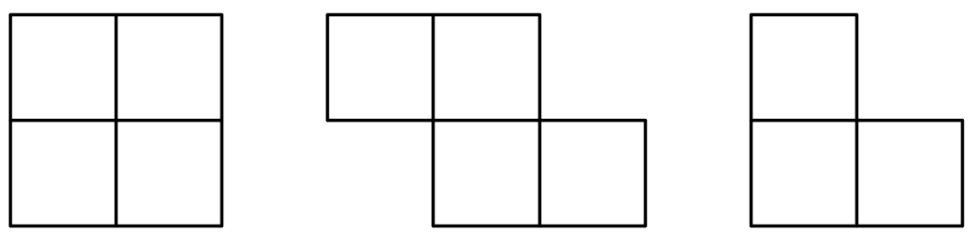
\includegraphics[height=1cm]{kacheln3.png}
\end{figure}

\bigskip
\end{enumerate}


\vspace{1.5cm} 

\center{Bonne chance!}
\end{document}
